\section{V12, Serielle Schnittstelle}
\subsection{Grundlagen}
\subsubsection{Serielle vs. Parallele Daten"ubertragung}
\begin{minipage}{12cm}
	Bei einem seriellen Kommu nikationskanal werden die einzelnen Datenbits sequenziell hintereinander "uber eine Signalleitung "ubertragen. Im Gegensatz dazu k"onnen bei einem parallel Kommunikationskanal mehrere Datenbits auf einmal transferiert werden. Sowohl bei der seriellen wie auch bei der parallelen "Ubertragung ist dabei immer eine bestimmte Bit-"Ubetragungszeit $t_{bit}$ einzuhalten.
	
	Bei seriellen Kommunikationskan"alen werden allgemein zwei unterschiedliche Metriken unterschieden, die \textit{Bit Rate} und die \textit{Baud Rate}.
	
	Die \textit{Bit Rate} sagt aus, wie viele \textit{bits-per-second} oder \textit{bts} "uber den Datenkanal transferiert werden k"onnen.
	
	Die \textit{Baud Rate} sagt aus, wie viele sogennante \textit{Symbols} sich in einer Sekunde "uber den Datenkanal transferieren lassen. Ist jedes Symbol durch ein Bit repr"asentiert spricht man von einer \textit{Dualen Codierung} (Bit/s = bps $\equiv$ Baud)
\end{minipage}
%
\begin{minipage}{0.5cm}
	\-\
\end{minipage}
%
\begin{minipage}{6cm}
	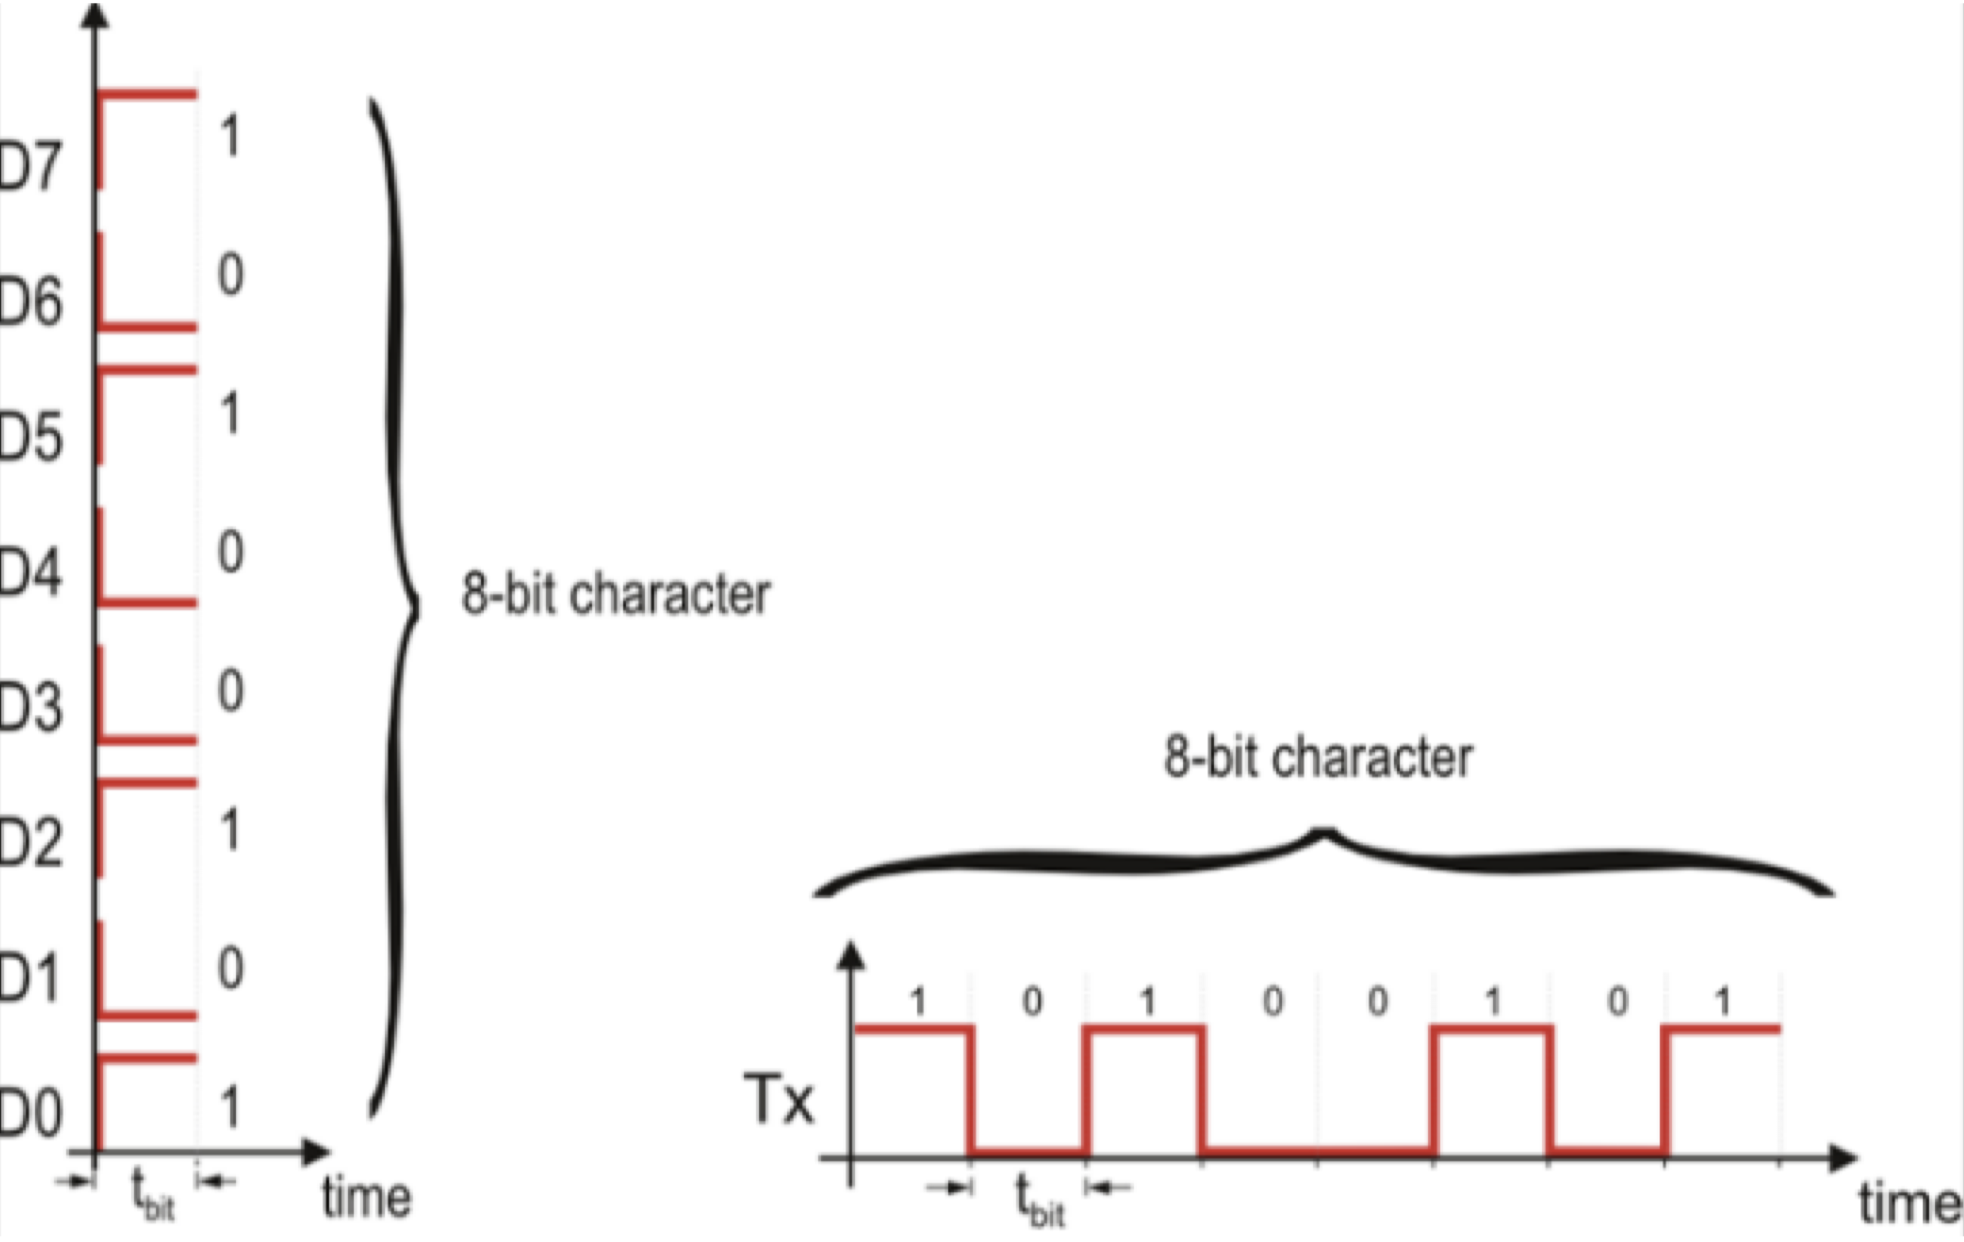
\includegraphics[width=6cm]{images/serielle-parallel_grundlagen}
\end{minipage}

\subsubsection{Parallel-Seriell Umsetzung}
Der Mikroprozessor verarbeitet die Daten intern in aller Regel parallel. F"ur die serielle Daten"ubertragung ist daher eine koordinierte Parallel-Serien-Wandlung in eine daf"ur vorgesehenen I/O-Port erforderlich.
	\begin{center}
		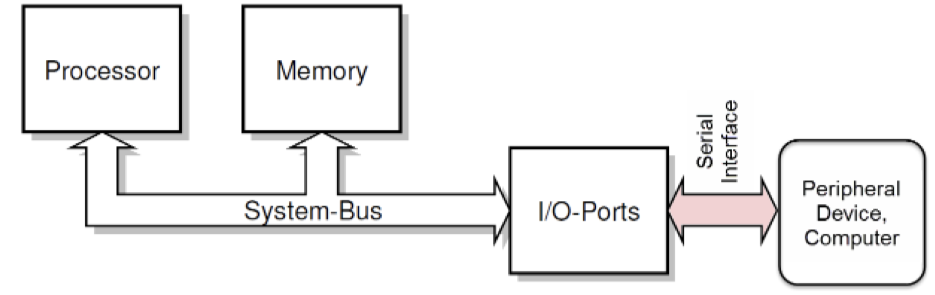
\includegraphics[width=12cm]{images/seriell_parallel}
	\end{center}
	
\subsubsection{Aufbau von Datenkan"alen}Kommunikatiosnkan"ale k"onnen auf verschiedene Arten implementiert werden. So k"onnen drahtgebundene Kan"ale beispielsweise als \textit{Single-Ended} oder als \textit{Differential Link} umgesetzt werden.\\
	
	\begin{minipage}[t]{9cm}
		\textbf{Single Ended (a)}\\
		Bei einer Single-Ended Verbindung werden einzelne, getrennte Signalleitungen ben"otigt, sowie eine Referenzleitung mit Ground-Potenzial
	\end{minipage}
	%
	\begin{minipage}[t]{0.5cm}
		\-\
	\end{minipage}
	%
	\begin{minipage}[t]{9cm}
		\textbf{Differential Link (b)}\\
		Bei einer Differential Verbindung wird der Datenlink durch eine Differenzspannung zwischen zwei zusammengeh"orenden Signalleitungen V(+) und V(-) repr"asentiert. Dies ist deutlich robuster als Single-Ended. F"ur eine serielle Differential Datenschnittstelle gen"ugen insgesamt drei Leitungen.
	\end{minipage}
	
	\begin{center}
		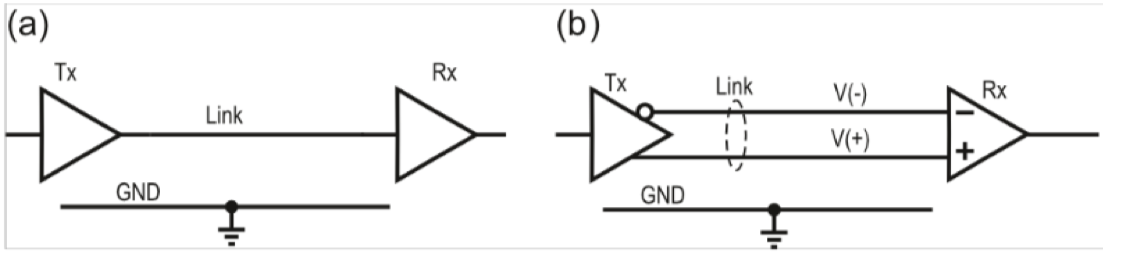
\includegraphics[width = 16cm]{images/diff_link}
	\end{center}

\newpage
\subsubsection{Simplex, Half- und Full-Duplex}
Datenkan"ale werden mit \textit{Simplex, Half-Duplex} oder \textit{Full-Doplex} bezeichnet, je nach Art der Konektivit"at.

		\textbf{Simplex}\\
		Ein Simplex serieller Kanal "ubertr"agt permanent in nur einer Richtung, "uber eine dedizierte Verbindung. An einem Ende des Kommunikationskanals arbeitet ein
			Transmitter, w"ahrend auf der anderen Seite ein Receiver steht. Simplex Kan"ale haben keine M"oglichkeit, den Empfang der Daten zu quittieren.
		\begin{center}
			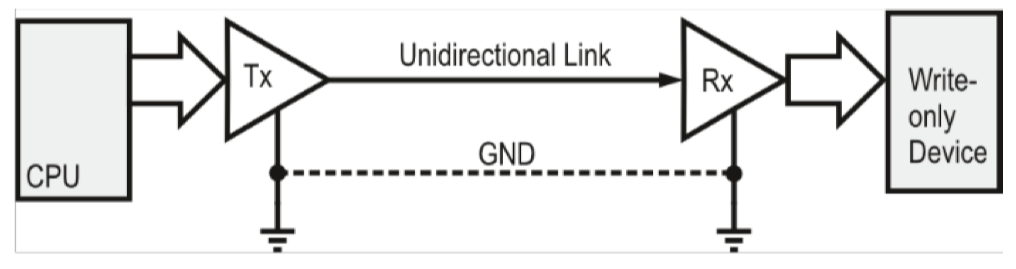
\includegraphics[width=12cm]{images/Simplex_serial}
		\end{center}
		

		\textbf{Half-Duplex}\\
		Ein Half-Duplex serieller Kanal verf"ugt ebenfalls nur "uber eine einzige Verbindung. Diese erlaubt jedoch eine beidseitige Kommunikation, aber nur in einer Richtung zur gleichen Zeit. Auf beiden Seiten des Kommunikationskanals steht ein serieller Transceiver, der sowohl als Sender wie auch als Empf"anger arbeiten kann. Wird die "Ubertragungsrichtung ge"andert, so mu"ussen die beiden Transceiver ihre Betriebsart wechseln. Das Umschalten der Datenrichtung erfordert klare Regeln auf beiden Seiten, um beispielsweise ein gleichzeitiges Senden zu vermeiden.
		\begin{center}
			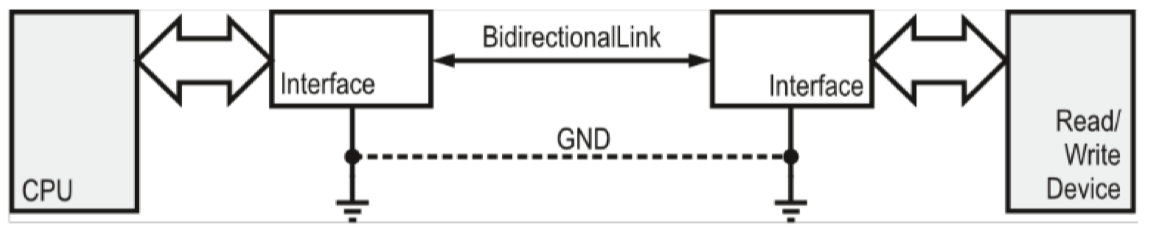
\includegraphics[width=12cm]{images/half_duplex}
		\end{center}
		
	 
	 	\textbf{Full-Duplex}\\
	 	Full-Duplex serielle Kan"ale verf"ugen "uber zwei separate Datenlinks; einer um Daten zu senden und ein anderer um Daten zu empfangen. Damit ist eine gleichzeitige Kommunikation in beide Richtungen m"oglich. Auf beiden Seiten des Kommunikationskanals steht ein serieller Transceiver, der zeitgleich als Sender und Empf"anger arbeitet.
	 	\begin{center}
			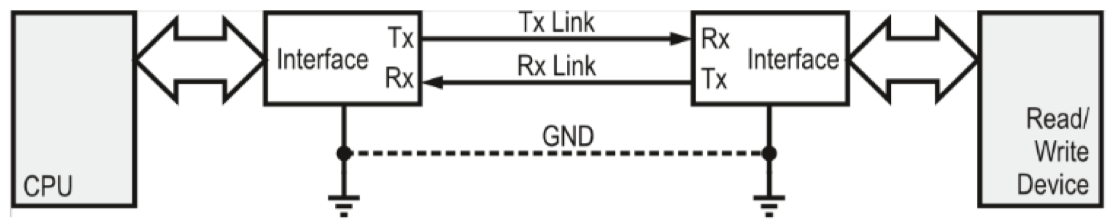
\includegraphics[width=12cm]{images/full_duplex}
		\end{center}

\newpage
\subsection{Synchrone Daten"ubertragung}
Synchrone serielle Kan"ale werden dadurch gekennzeichnet, dass Sender und Empf"anger auf das gleiche Clock-Signal synchronisiert sind $\Rightarrow$ zus"atzliche Clock-Leitung. Synchrone Kan"ale arbeiten "ublicherweise in einer \textit{Master/Slave-Beziehung}.\\
	\begin{center}
		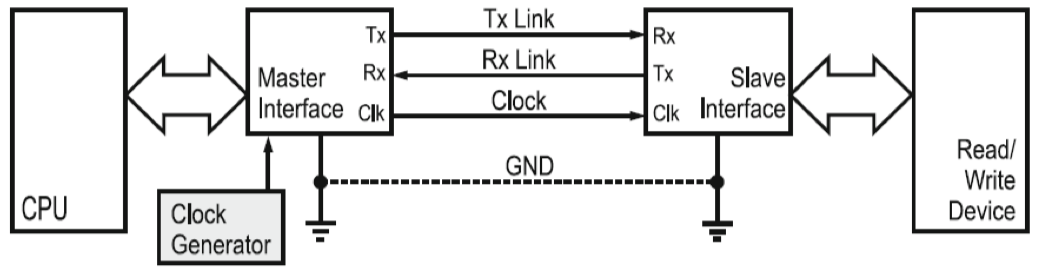
\includegraphics[width=12cm]{images/synch_full_duplex}
	\end{center}
	
\subsubsection{Daten"ubertragung}
Beim der synchronen seriellen Datenkanal werden die Daten typischerweise in Bl"ocken mit variabler L"ange "ubertragen. Parallel dazu erfolgt die "Ubertragung der Clock Information. Dabei ist wichtig, dass Sender und Empf"anger auf die gleiche Flanke Daten "ubernehmen.

Im folgenden Bild ist exemplarisch eine ganze Message mit drei Data Packets (Datagrams) dargestellt: Das Synchronisationszeichen (Sync) kennzeichnet als Header den Beginn eines zusammengeh"orenden Data Pakets. Grunds"atzlich wird nach jedem Datenblock (Body) das Zeichen ETB (End of Transmission Block) als Footer "ubertragen. Das Ende der gesamten Message wird durch ein EOT (End of Transmission) gekennzeichnet. Das ETB kann vor einem EOT je nach Protokoll entfallen.
	\begin{center}
		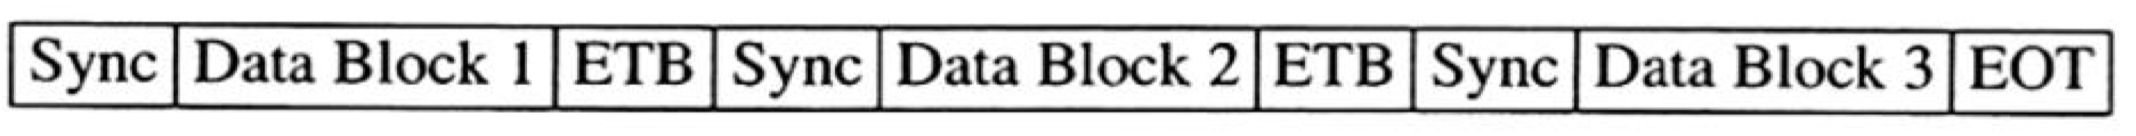
\includegraphics[width=12cm]{images/synch-serielle-data-bsp}
	\end{center}

\subsection{Asynchrone Daten"ubertragung}
Beim asynchronen seriellen Datenkanal laufen auf der Sender- und Empf"angerseite zwei unabh"angige Clock-Generatoren. Dabei m"ussen diese auf die selbe Baud-Rate eingestellt werden. 
	\begin{center}
		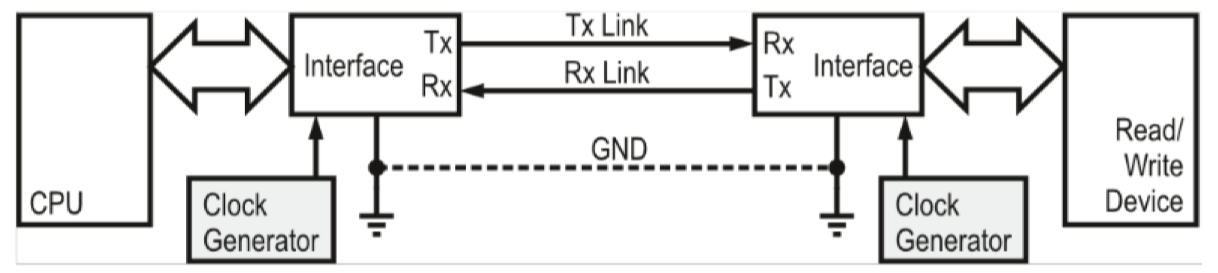
\includegraphics[width=12cm]{images/asynch_serial.png}
	\end{center}

Auf die fallende Datenflanke des Datenframes wird der jeweilige Clock-Generator synchronisiert. Dabei haben Datenpakete folgenden Aufbau:\\
	\begin{minipage}{11cm}
		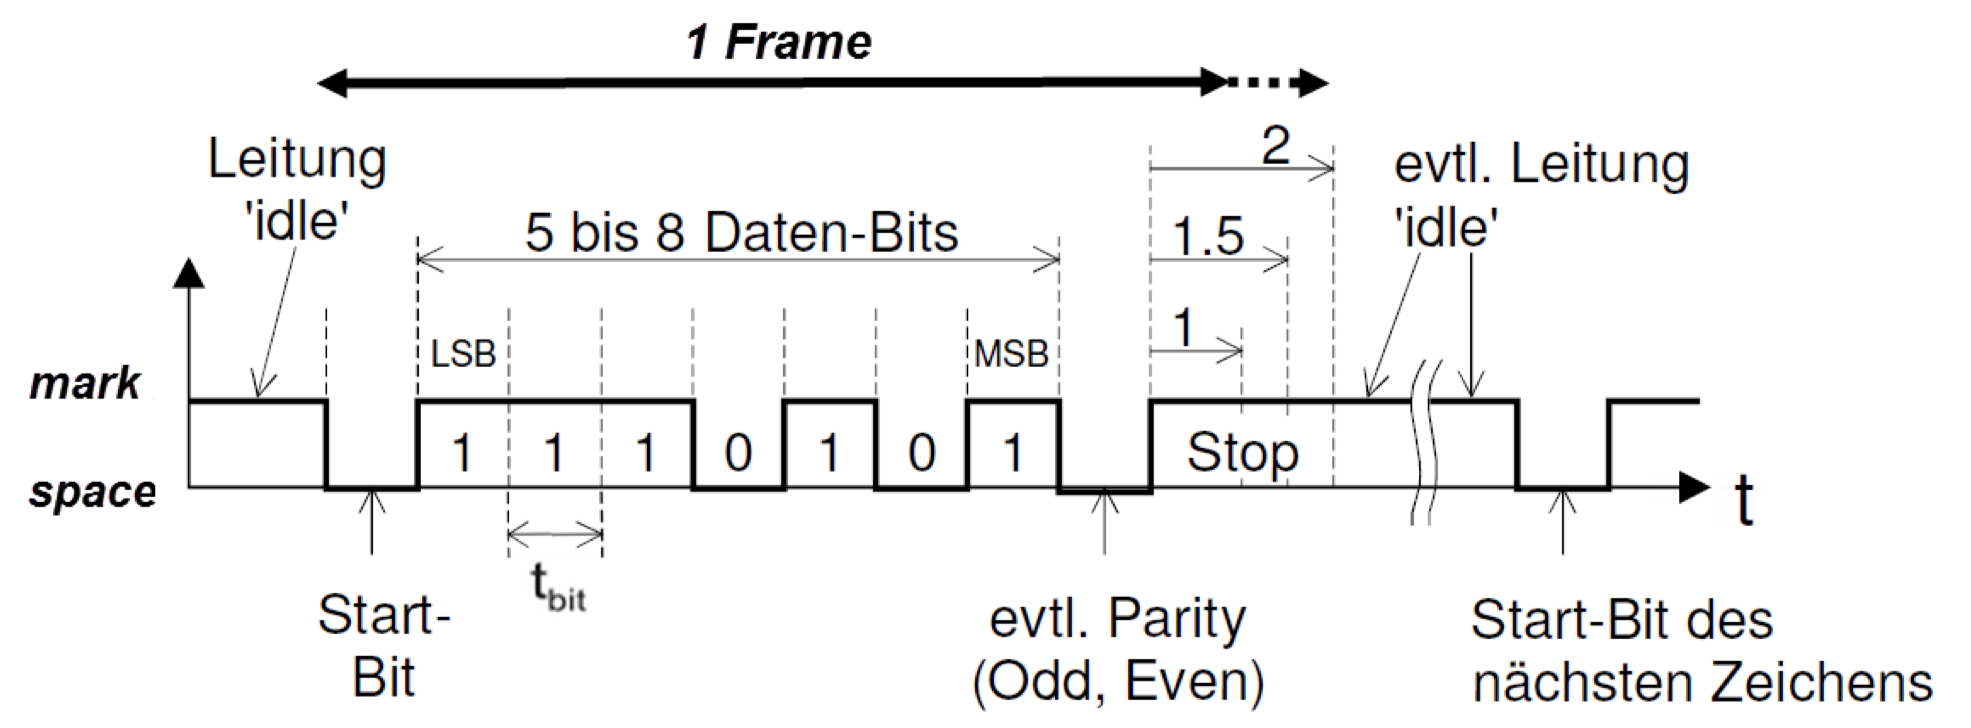
\includegraphics[width=11cm]{images/datenframe-uart}\\
		Datenframe einer UART Schnittstelle (7-Bit, Odd Parity)
	\end{minipage}
	%
	\begin{minipage}{0.5cm}
		\-\
	\end{minipage}
	%
	\begin{minipage}{7cm}
		Die beteiligten Kommunikationsschnittstellen ben"otigen folgende Informationen um ihre Interfaces auf den asynchronen seriellen Bitstrom abzustimmen:
		\begin{itemize}
			\item Baudrate = $\frac{1}{t_{bit}}$
			\item Anzahl Daten-Bits (5 bis 8)
			\item Parity Information (Even / Odd / none) Das Paritybit erg"anzt immer auf \textit{Odd} oder \textit{Even}.
			\item Anzahl Stop-Bit (1 / 1.5 / 2)
		\end{itemize}
	\end{minipage}\\

Aus den Informationen der Kommunikationsschnittstelle l"asst sich zudem die Nutzdatenrate bestimmen.
	\begin{equation*}
		Nutzdatenrate = \frac{\#Databit \cdot Baudrate}{\#Startbit + \#Databit + \#Paritybit + \#Stopbit} \cdot \frac{1 Byte}{8 Bit}
	\end{equation*}
	
\newpage
\subsubsection{Datenflusssteuerung}
Bei der seriellen Kommunikation muss oft der Datenfluss gesteuert werden. Dies ist zum Beispiel dann dringend notwendig, wenn empf"angerseitig der Datenpuffer voll wird und ein Daten"uberlauf droht. Dieser Zustand muss an den Datensender signalisiert werden. $\Rightarrow$ HW- und SW-Handshake\\

	\begin{minipage}[t]{9cm}
		\textbf{Hardware Handshaking}\\
		Mit Hardware-Signalen teilen sich die Kommunikationspartner gegenseitig mit, ob sie bereit sind weitere Daten aufzunehmen oder nicht.
		\begin{center}
			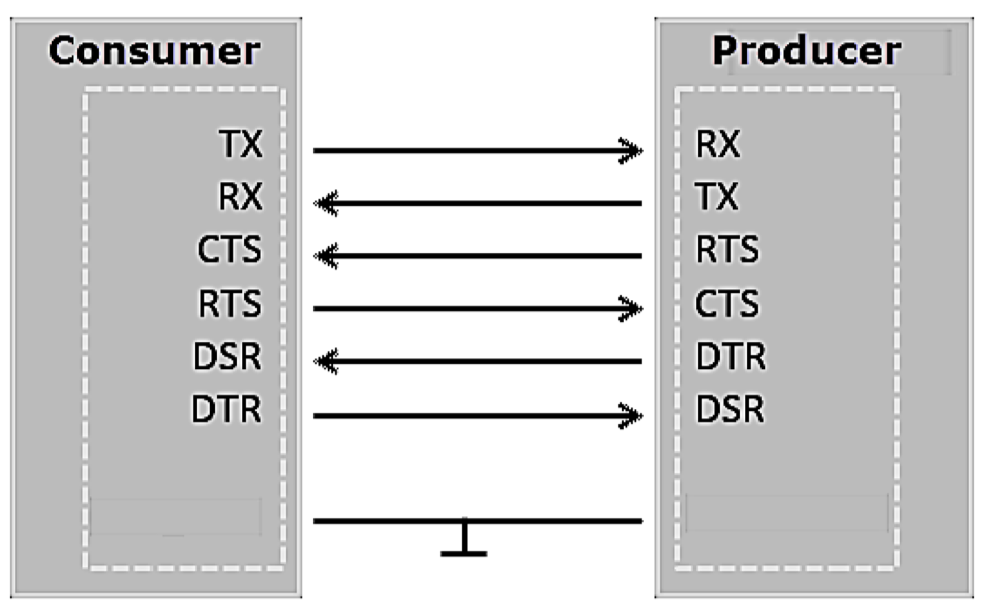
\includegraphics[width=5cm]{images/HW-handshake}\\
			\textit{RTS (request to send), CTS (clear to send)}
		\end{center}
	\end{minipage}	
	%
	\begin{minipage}[t]{0.5cm}
		\-\
	\end{minipage}
	%
	\begin{minipage}[t]{9cm}
		\textbf{Software Handshaking}\\
		Beim Software Handshaking kommen anstelle von zus"atzlichen Handshake-Leitungen zwei extra f"ur diesen Zweck reservierte ASCII-Zeichen zur Anwendung:
		\begin{itemize}
			\item \textbf{XON} ASCII DC1 0x11
			\item \textbf{XOFF} ASCII DC3 0x13
		\end{itemize}
		\begin{center}
			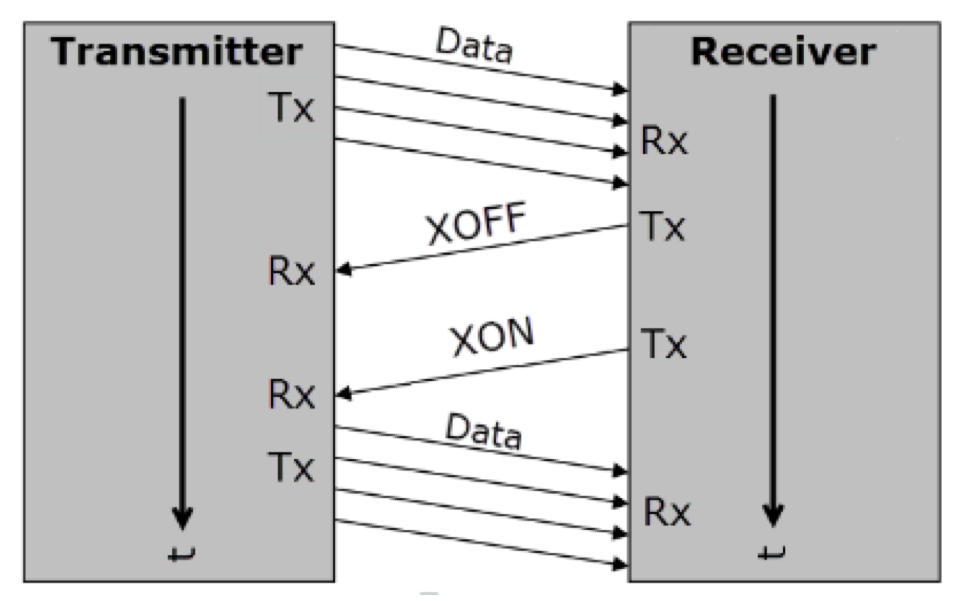
\includegraphics[width=5cm]{images/SW-handshake}
		\end{center}
	\end{minipage}
\subsection{Standardisierte serielle Interfaces}
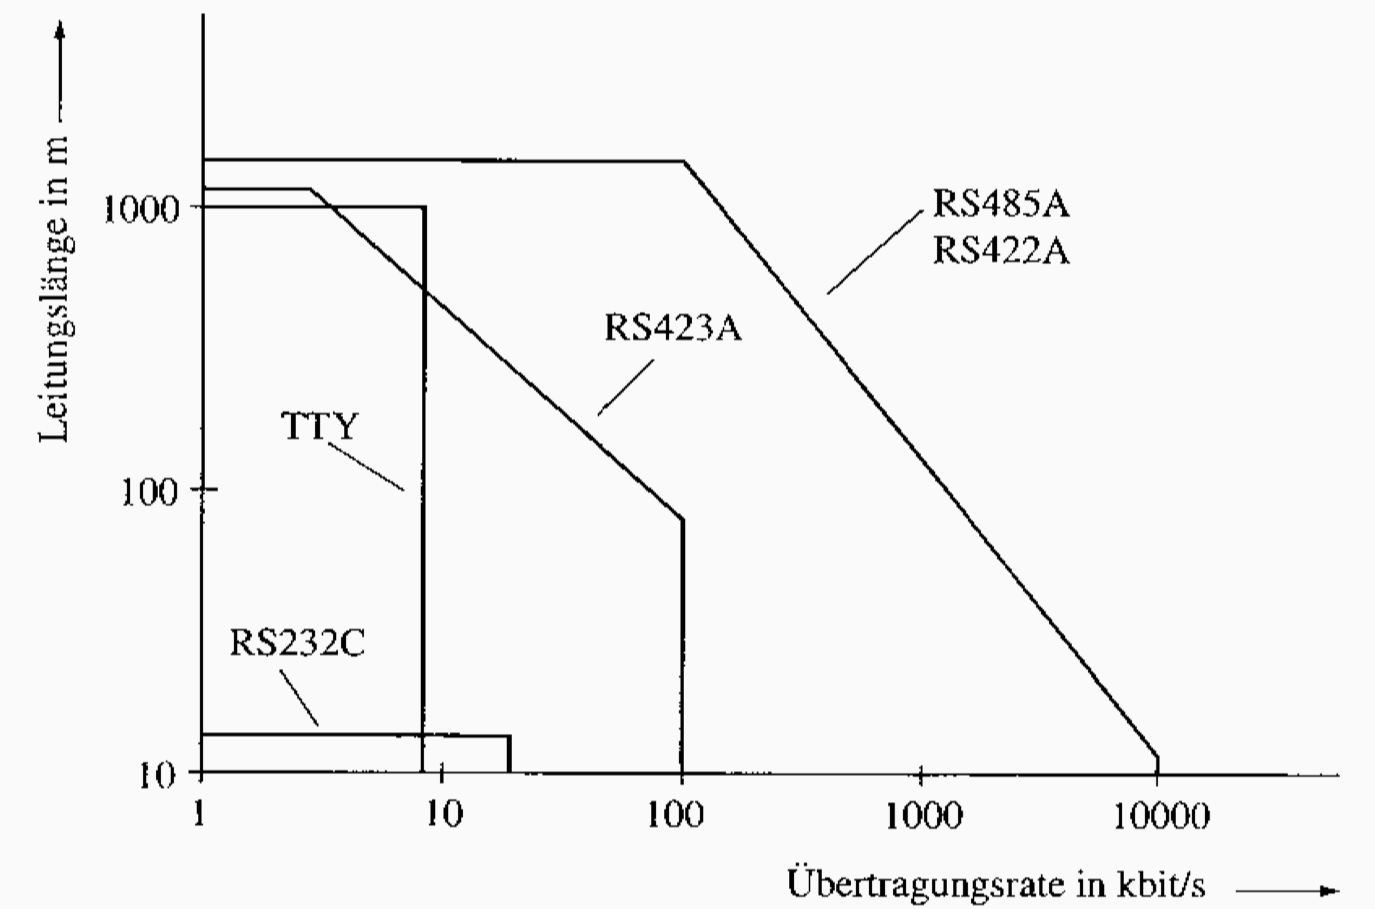
\includegraphics[width=7cm]{images/uebertragungsraten_seriellen_schnittstellen}
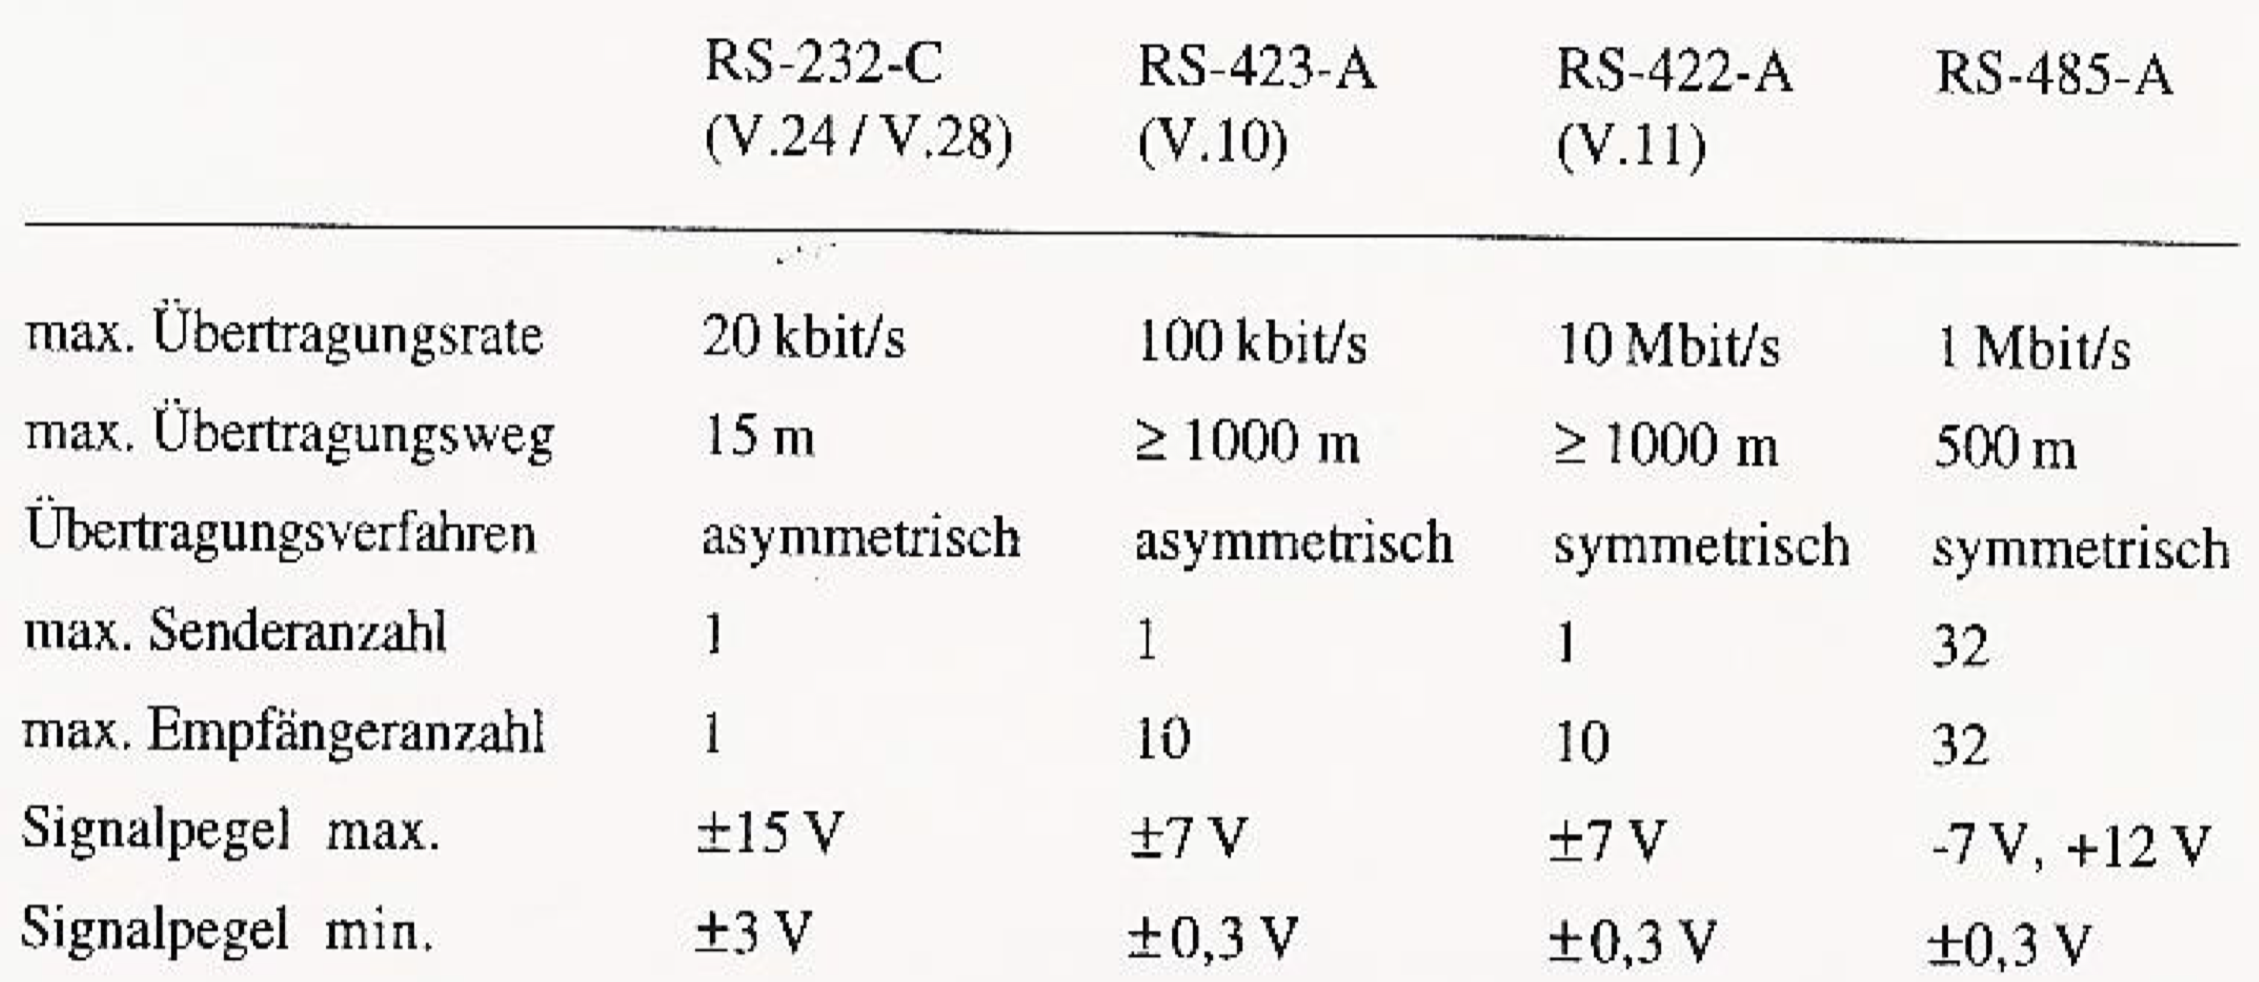
\includegraphics[width=11cm]{images/uebersicht-serielle-schnittstellen}